\chapter{Überwachtes Lernen}
\label{subsec:lean}
Beide unbewachte Ansätze erwiesen sich als nicht zufriedenstellend, dennoch haben sie wertvolle Erkenntnisse geliefert. Es wurde festgestellt, dass die erforderlichen Korrelationswerte für eine Evaluierung vorhanden sind, mit Ausnahme von neuen Hotels ohne entsprechende Daten. Nichtsdestotrotz könnten die bestehenden Korrelationswerte trotzdem genutzt werden, um ein Modell zu trainieren. Die Idee besteht darin, die beschreibenden Merkmale eines Hotels in ein trainiertes Modell einzuspeisen, um die Korrelationswerte vorherzusagen, anstatt direkt ähnliche Hotels zu prognostizieren.
\newline
\newline
Konkret sieht der Ansatz wie folgt aus: Jedes Hotel im Datensatz wird mit jedem anderen Hotel kombiniert, wodurch ein Datensatz der Größe \emph{Anzahl der Hotels x Anzahl der Hotels} entsteht. Zu jeder Kombination wird der Korrelationswert in einer separaten Spalte hinzugefügt, die als Zielvariable für die Vorhersage dient. Ein Modell wird mithilfe dieser Daten und der jeweiligen Zielvariable trainiert. Bei der Vorhersage der Korrelationswerte für ein neues Hotel wird dieses mit jedem anderen Hotel kombiniert und in das Modell eingebracht. Das Modell gibt schließlich die vorhergesagten Korrelationswerte aus.
\newline
\newline
Um diese theoretische Idee zu konkretisieren, werden im folgenden Abschnitt die einzelnen Schritte veranschaulicht.

\section{Vorbereitung des Datensatzes}
\label{subsubsec:learn_prepare}
Um die beschriebene Idee in die Tat umzusetzen, bedarf es zunächst einer Modifikation des Datensatzes, welcher in Abbildung \ref{img:all_features_4} dargestellt ist. Jede Zeile soll mit jeder anderen Zeile kombiniert werden. Dies wird durch die nachfolgenden Codezeilen realisiert:

\begin{lstlisting}[language=Python, label=lst:learn_prepare, caption=Erstellen des kombinierten Datensatzes]
# Get Hotel ID as seperate column
model_df = model_df.reset_index()
    
# Repeat the rows 2 times
repeat = 2
    
# Get all row combinations 
combinations = list(product(model_df.index, repeat=repeat))
    
# Create the empty result dataframe
combined_df = pd.DataFrame(columns=[f"{column}_{i+1}" for i in range(repeat) for column in model_df.columns])
    
# Combine all combinations in the result dataframe
for combination in combinations:
    row1 = model_df.iloc[combination[0]].values
    row2 = model_df.iloc[combination[1]].values
    new_row = pd.Series(list(row1) + list(row2), index=combined_df.columns)
    combined_df = combined_df.append(new_row, ignore_index=True)
\end{lstlisting}

Mithilfe der im Listing \ref{lst:learn_prepare} präsentierten Codezeilen wurden sämtliche Zeilen erfolgreich miteinander kombiniert. Anschließend kann der Korrelationswert jeder Kombination als neue Spalte \emph{target} hinzugefügt werden.
\newline
\newline
Der resultierende Datensatz, welcher für das Modell verwendet werden soll, sieht wie folgt aus\footnote{Die Hotel-IDs wurden zur besseren Veranschaulichung entfernt}:

\begin{figure}[h]
    \centering
    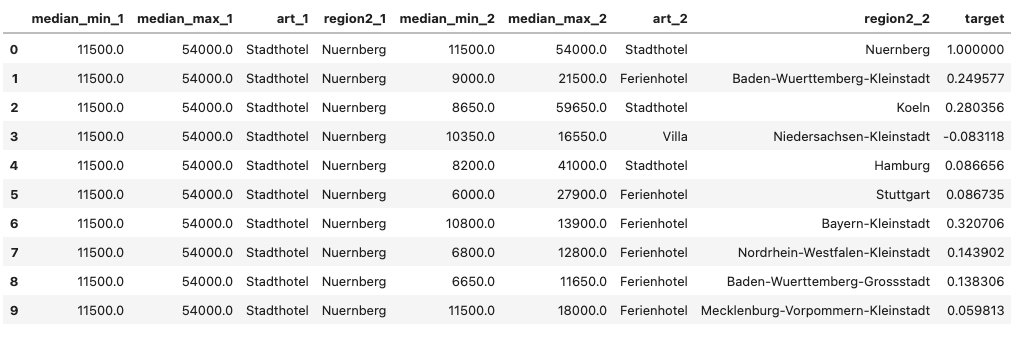
\includegraphics[width=1\textwidth, center]{learn_df1.png}
    \caption[Datensatz bestehend aus den einzelnen Kombinationen]{Datensatz bestehend aus den einzelnen Kombinationen}
    \label{img:learn_df1}
\end{figure}

\section{Modellbildung}
\label{subsubsec:learn_model}
Für das überwachte Lernen wird CatBoost verwendet, ein hochentwickelter Machine-Learning-Algorithmus, der gezielt auf die Vorhersage von kategorialen Variablen in Datensätzen abzielt und auf dem Gradient Boosting Framework basiert. Eine signifikante Eigenschaft von CatBoost ist seine einzigartige Methode zur Behandlung von kategorialen Merkmalen, bekannt als \emph{Kategorie-Binning}. Diese Methode befähigt den Algorithmus dazu, die internen Strukturen kategorialer Variablen besser zu erfassen und sie effektiv in den Trainingsprozess einzubeziehen, was zu präziseren Vorhersagen führt \cite{Hancock.2020}.
\newline
\newline
Angesichts der Fülle an kategorialen Variablen im vorliegenden Datensatz erweist sich der CatBoost-Algorithmus als besonders geeignet für diese spezifische Aufgabe. Demzufolge kann der Datensatz in seiner aktuellen Form verwendet werden, ohne dass eine umfangreiche Vorverarbeitung erforderlich ist.
\newline
\newline
Im folgenden Abschnitt werden die erforderlichen Codezeilen präsentiert, um das Modell zu trainieren und Vorhersagen für das Benchmark-Hotel zu generieren:

\begin{lstlisting}[language=Python, label=lst:learn_model_train, caption=Erzeugung der Vorhersagen von ähnlichen Hotels mittels CatBoost]
# Get test data
test = combined_df[combined_df["company_id_1"] == str(benchmark_hotel_id)]
# Get train data
train = combined_df.drop(combined_df[(combined_df["company_id_1"] == str(benchmark_hotel_id)) | (combined_df["company_id_2"] == str(benchmark_hotel_id))].index)
# Get X and y from test and train
y_train = train["target"]
X_train = train.drop("target", axis=1)
y_test = test["target"]
X_test = test.drop("target", axis=1)
# Save important informations
hotel_test_df = X_test[["company_id_1", "company_id_2"]]
hotel_test_df["target"] = list(y_test)
# Drop Company ID
X_train = X_train.drop(['company_id_1', "company_id_2"], axis=1)
X_test = X_test.drop(['company_id_1', "company_id_2"], axis=1)
# Define cat features 
cat_features = ["art_1", "region2_1", "art_2","region2_2"]
# Define and train model 
model = cb.CatBoostRegressor()
model.fit(X_train, y_train, cat_features=cat_features)
# Get predictions 
y_pred = model.predict(X_test)
# Add predictions to the information df
hotel_test_df["predictions"] = list(y_pred)
\end{lstlisting}

Mithilfe der Codezeilen im Listing \ref{lst:learn_model_train} wurde ein zusätzliches DataFrame erstellt, das die Hotel-IDs sowie deren Vorhersagen enthält. Dieses DataFrame wird im Folgenden präsentiert:

\begin{figure}[h]
    \centering
    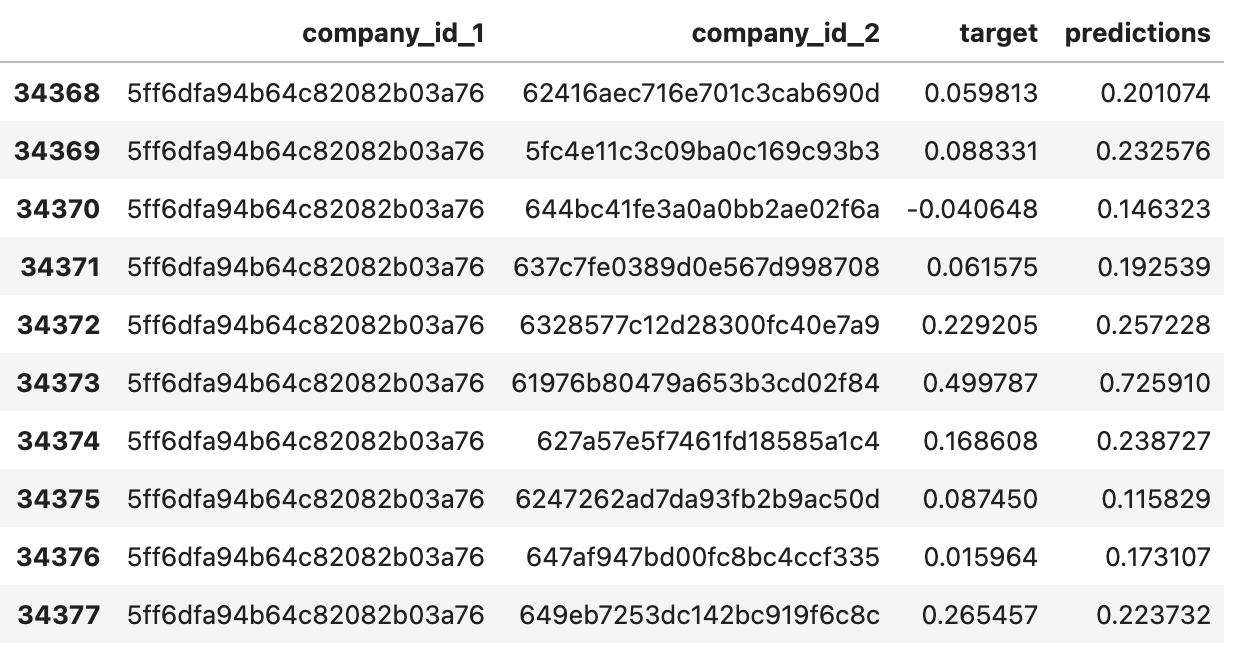
\includegraphics[width=1\textwidth, center]{catboost_similar_results.png}
    \caption[Datensatz der Hotel-IDs und deren Korrelationswert]{Datensatz der Hotel-IDs und deren Korrelationswert}
    \label{img:catboost_similar_results}
\end{figure}

Es besteht nun die Möglichkeit, verschiedene Operationen auf dem DataFrame auszuführen. Zum Beispiel kann auf dem DataFrame gemäß der Bedingung in Abschnitt \emph{\nameref{subsec:un_lear}} gefiltert werden, die besagt, dass Hotelkorrelationen mit mindestens einem Korrelationswert von 0,8 gefunden werden sollen.

\section{Evaluation}
\label{subsubsec:learn_eval}
Im Gegensatz zu früheren Modellen wurde bei diesem Modell auf eine umfassende Evaluation verzichtet, da der prognostizierte Korrelationswert ausreichend ist, um ähnliche Hotels zu identifizieren. Es wurde lediglich versucht, den R2-Score mithilfe von Hyperparameteranalysen mittels Random Search 
\cite{AdapRandomSearch4.05.2009} und Grid Search \cite{Liashchynskyi.12.12.2019} zu verbessern.


